\chapter{PK1 --- Tài khoản \& bảo mật}
\begin{figure}[H]\centering
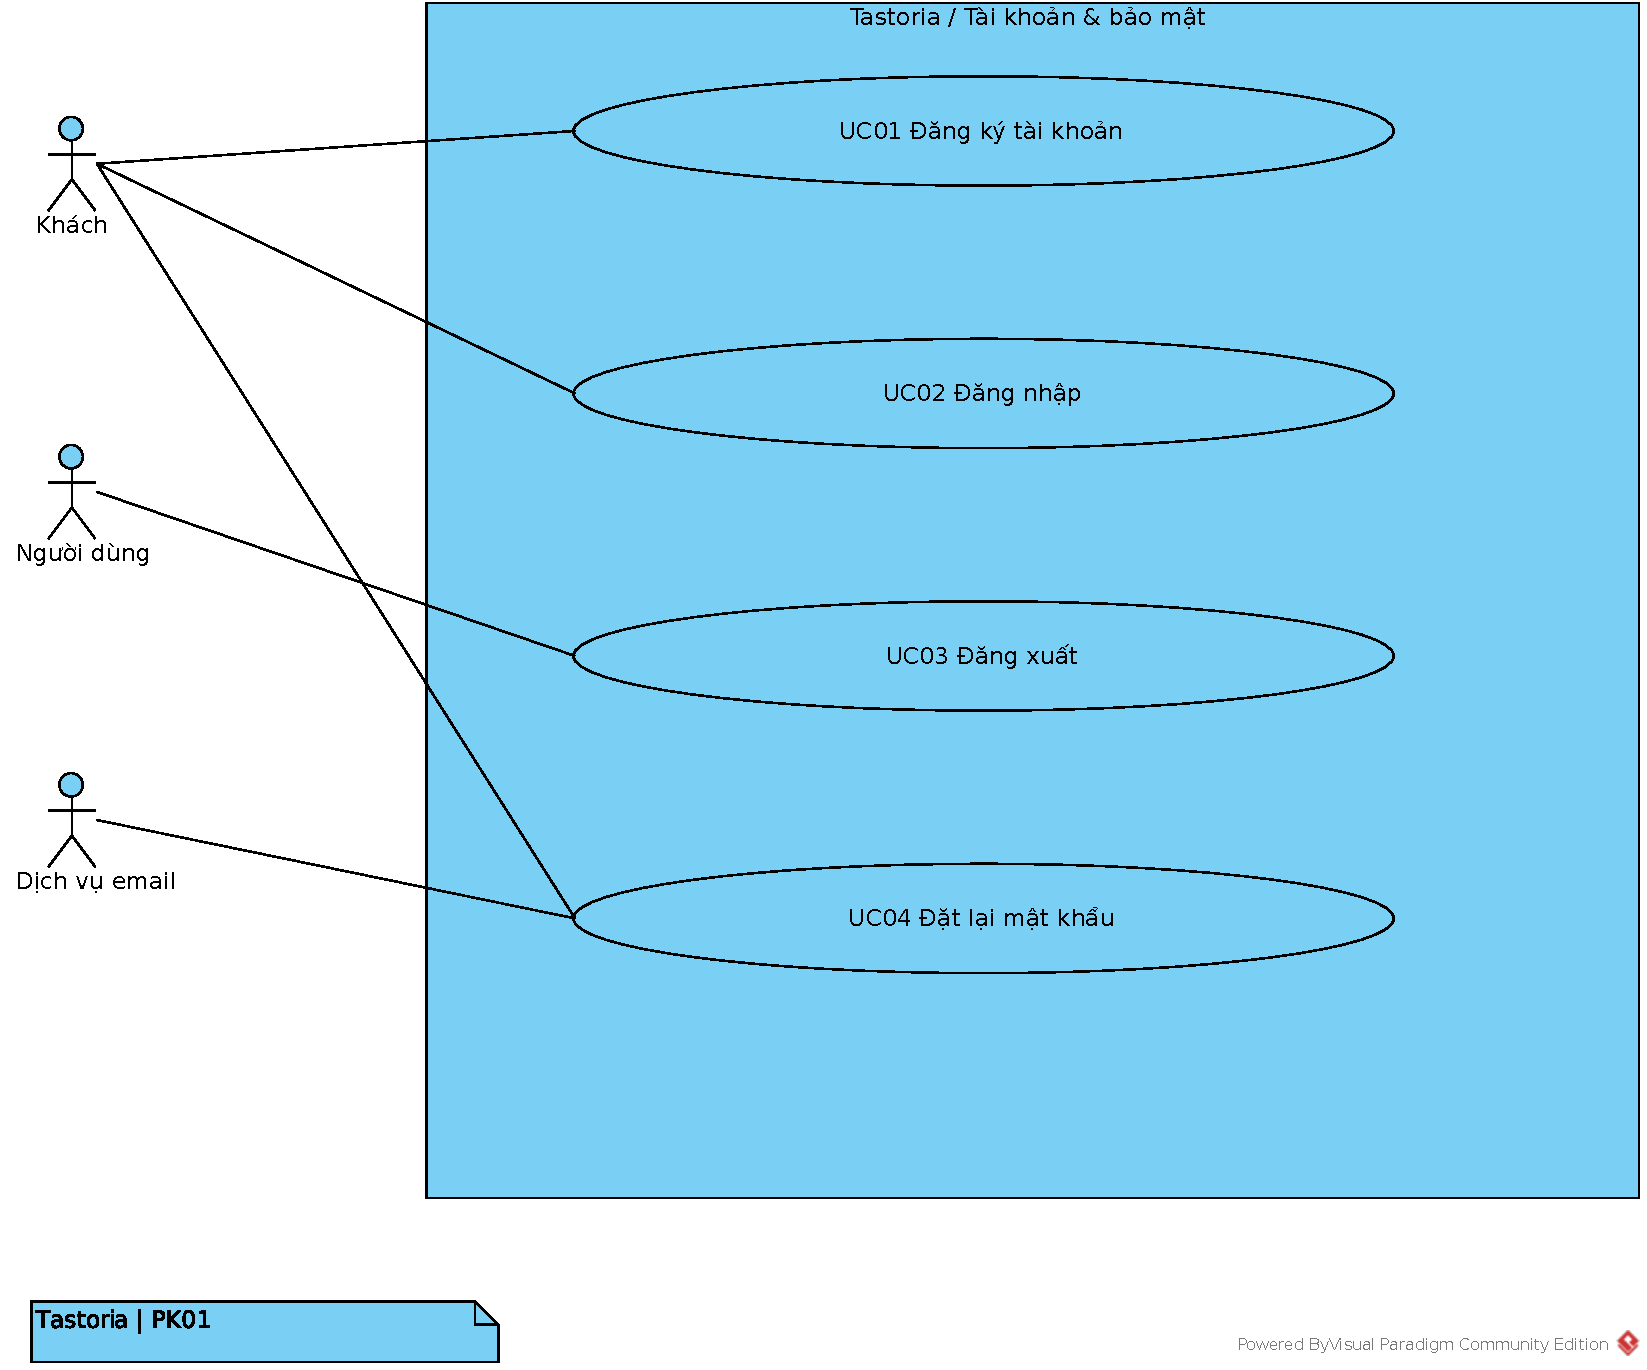
\includegraphics[width=0.96\linewidth,height=0.75\textheight,keepaspectratio]{assets/PK01.pdf}
\caption{PK01 --- Phân rã use case}\label{fig:Phu-luc-A-Use-Cases:1}
\end{figure}
\section{UC01 --- Đăng ký tài khoản}
\subsection{Mục tiêu trong ngữ cảnh}
Khách (A01) tạo tài khoản bằng email và mật khẩu để dùng các chức năng cần đăng nhập (hồ sơ, kho, mâm cơm). Sau khi đăng ký, người đó trở thành Người dùng (A02) và được chuyển sang thiết lập hồ sơ (UC09).

\subsection{Phạm vi và mức}
\begin{itemize}
\item Phạm vi: hệ thống Tastoria (app Android/\allowbreak{}web + backend), module {\small\texttt{identity}} (M02).
\item Mức: mục tiêu người dùng (user goal), một phiên làm việc dưới 1 phút.
\item Không thuộc UC này: thu đồng ý theo mục đích (thuộc UC05, được sử dụng có điều kiện trong UC09), nhập hồ sơ (UC09).
\end{itemize}
\subsection{Tác nhân và bên liên quan (quyền lợi)}
{\footnotesize\setlength{\tabcolsep}{0pt}
\begin{longtable}{@{}L{7.850cm}@{\hspace{3mm}}L{7.850cm}@{}}
\caption{Tác nhân và bên liên quan (quyền lợi)}\\
\toprule
\textbf{Tác nhân /\allowbreak{} bên liên quan} & \textbf{Quyền lợi} \\
\midrule\endfirsthead
\multicolumn{2}{l}{\small\itshape Bảng \thetable{} (tiếp theo)}\\
\toprule
\textbf{Tác nhân /\allowbreak{} bên liên quan} & \textbf{Quyền lợi} \\
\midrule\endhead
\bottomrule\endfoot
A01 Khách (chính) & Tạo tài khoản nhanh, không bị hỏi dữ liệu chưa cần; biết ngay nếu email đã dùng. \\ \addlinespace[3pt]
Nhóm vận hành Tastoria & Mỗi email đúng một tài khoản; mật khẩu không bao giờ lưu dạng rõ. \\ \addlinespace[3pt]
Chủ thể dữ liệu (chính A01) & Không có đồng ý nào bị ghi thay mình trong lúc đăng ký (BR-\allowbreak{}CONSENT-\allowbreak{}01). \\ \addlinespace[3pt]
\end{longtable}}
\subsection{Tiền điều kiện}
\begin{itemize}
\item Khách chưa đăng nhập trên thiết bị.
\item App kết nối được tới {\small\texttt{/\allowbreak{}\allowbreak{}api/\allowbreak{}\allowbreak{}v1}}.
\end{itemize}
\subsection{Đảm bảo tối thiểu}
\begin{itemize}
\item Không có tài khoản dở dang: hoặc có đủ bản ghi {\small\texttt{users}} (và token nếu cấp), hoặc không có gì.
\item Mật khẩu không xuất hiện dạng rõ trong CSDL, log hay phản hồi.
\item Không có bản ghi {\small\texttt{consent\_\allowbreak{}\allowbreak{}events}} nào được tạo.
\end{itemize}
\subsection{Đảm bảo khi thành công}
\begin{itemize}
\item Có một dòng {\small\texttt{users}} mới: {\small\texttt{role = user}}, {\small\texttt{status = active}}, {\small\texttt{token\_\allowbreak{}\allowbreak{}version = 0}}, {\small\texttt{failed\_\allowbreak{}\allowbreak{}logins = 0}}, {\small\texttt{password\_\allowbreak{}\allowbreak{}hash}} dạng Argon2id.
\item App nhận access token và refresh token của phiên đầu tiên (một {\small\texttt{refresh\_\allowbreak{}\allowbreak{}tokens}} mới với {\small\texttt{family\_\allowbreak{}\allowbreak{}id}} mới) và chuyển sang UC09.
\end{itemize}
\subsection{Kích hoạt}
Khách chọn "Đăng ký" trên màn Đăng ký/\allowbreak{}Đăng nhập.

\subsection{Kịch bản chính}
\begin{enumerate}
\item A01 mở màn Đăng ký, nhập email và mật khẩu (ô mật khẩu có nút hiện/\allowbreak{}ẩn).
\item App kiểm tra cú pháp email và độ dài mật khẩu phía client, rồi gửi {\small\texttt{POST /\allowbreak{}\allowbreak{}auth/\allowbreak{}\allowbreak{}register}}.
\item Module {\small\texttt{identity}} chuẩn hoá email (cắt khoảng trắng; so khớp không phân biệt hoa thường nhờ kiểu {\small\texttt{citext}}) và kiểm tra chính sách mật khẩu.
\item Module {\small\texttt{identity}} băm mật khẩu bằng Argon2id ({\small\texttt{pwdlib}}).
\item Module {\small\texttt{identity}} mở một giao dịch (Unit of Work của {\small\texttt{core}}), ghi {\small\texttt{users}}, tạo refresh token ngẫu nhiên, lưu {\small\texttt{token\_\allowbreak{}\allowbreak{}sha256}} vào {\small\texttt{refresh\_\allowbreak{}\allowbreak{}tokens}} với {\small\texttt{family\_\allowbreak{}\allowbreak{}id}} mới, {\small\texttt{expires\_\allowbreak{}\allowbreak{}at = issued\_\allowbreak{}\allowbreak{}at + 30 ngày}}, rồi commit.
\item Module {\small\texttt{identity}} ký access JWT 15 phút (có {\small\texttt{kid}}, mang {\small\texttt{token\_\allowbreak{}\allowbreak{}version}}) và trả 201 kèm hai token.
\item App lưu token vào secure-\allowbreak{}store và chuyển sang màn Hồ sơ 60 giây (UC09).
\end{enumerate}
\subsection{Mở rộng}
\begin{itemize}
\item \textbf{2a. Email sai cú pháp hoặc mật khẩu ngắn (kiểm phía client):} app đánh dấu ô lỗi bằng chữ, không gửi yêu cầu; quay lại bước 1.
\item \textbf{3a. Email sai cú pháp (kiểm phía server):} {\small\texttt{identity}} trả 422 {\small\texttt{application/\allowbreak{}\allowbreak{}problem+json}}, {\small\texttt{code = invalid\_\allowbreak{}\allowbreak{}email}}; không ghi gì; app hiện lỗi tại ô email.
\item \textbf{3b. Mật khẩu không đạt chính sách:} trả 422, {\small\texttt{code = weak\_\allowbreak{}\allowbreak{}password}}, kèm độ dài tối thiểu; không ghi gì.
\item \textbf{5a. Email đã có tài khoản:} ràng buộc UQ trên {\small\texttt{users.\allowbreak{}email}} từ chối; giao dịch rollback; trả 409, {\small\texttt{code = email\_\allowbreak{}\allowbreak{}taken}}. App đề nghị đăng nhập (UC02) hoặc đặt lại mật khẩu (UC04), email điền sẵn.
\item \textbf{5b. Hai yêu cầu đăng ký đồng thời cùng email:} ràng buộc UQ bảo đảm đúng một yêu cầu thành công; yêu cầu còn lại đi theo 5a.
\item \textbf{5c. Lỗi CSDL hoặc lỗi hệ thống:} giao dịch rollback; trả 500/\allowbreak{}503 problem+json có {\small\texttt{request\_\allowbreak{}\allowbreak{}id}}; không có tài khoản dở dang. App cho thử lại.
\item \textbf{*a. Mất mạng hoặc quá thời gian chờ phản hồi:} {\small\texttt{POST /\allowbreak{}\allowbreak{}auth/\allowbreak{}\allowbreak{}register}} không lũy đẳng. App gửi lại cùng email và mật khẩu. Nếu lần trước đã thành công, lần gửi lại nhận 409 {\small\texttt{email\_\allowbreak{}\allowbreak{}taken}} (5a); app khi đó tự gọi đăng nhập (UC02) với thông tin vừa nhập, nên kết quả cuối cùng vẫn là một tài khoản và một phiên.
\item \textbf{*b. Thiếu đồng ý:} không áp dụng ở UC này. Đăng ký không yêu cầu và không ghi đồng ý; đồng ý theo mục đích thu ở UC09 theo lựa chọn đồng ý từng mục đích.
\item \textbf{*c. Không khả thi:} không có nhánh không khả thi về nghiệp vụ.
\end{itemize}
\subsection{Ghi chú đối chiếu của báo cáo}
Giữ phạm vi yêu cầu của đặc tả nguồn; cần kiểm thử theo môi trường và phiên bản thực tế trước khi ghi kết quả nghiệm thu.

\textbf{Nguồn:} {\small\texttt{Tastoria/\allowbreak{}\allowbreak{}docs/\allowbreak{}\allowbreak{}sad/\allowbreak{}\allowbreak{}use-\allowbreak{}cases/\allowbreak{}\allowbreak{}UC01.\allowbreak{}md}}. Mã nghiệp vụ: BR-\allowbreak{}CONSENT-\allowbreak{}01.

\textbf{Dữ liệu liên quan:} {\small\texttt{users}}, {\small\texttt{refresh\_\allowbreak{}\allowbreak{}tokens}}, {\small\texttt{consent\_\allowbreak{}\allowbreak{}events}}.

\textbf{Điểm giao tiếp:} {\small\texttt{POST /\allowbreak{}\allowbreak{}auth/\allowbreak{}\allowbreak{}register}}.

\section{UC02 --- Đăng nhập}
\subsection{Mục tiêu trong ngữ cảnh}
Khách (A01) có tài khoản đăng nhập bằng email và mật khẩu để nhận phiên làm việc. UC này gồm cả làm mới phiên bằng refresh token (app tự gọi khi access token hết hạn) và khoá tạm khi nhập sai 5 lần (NFR-\allowbreak{}SEC-\allowbreak{}02).

\subsection{Phạm vi và mức}
\begin{itemize}
\item Phạm vi: hệ thống Tastoria, hộp đen.
\item Mức: mục tiêu con (subfunction). Đăng nhập không mang giá trị tự thân cho A01; nó phục vụ mọi UC cần tài khoản (quy tắc gán mức ở SRS \S{}2.2). Làm mới phiên là luồng phụ R của cùng UC, không phải kịch bản chính thứ hai.
\end{itemize}
\subsection{Tác nhân và bên liên quan (quyền lợi)}
{\footnotesize\setlength{\tabcolsep}{0pt}
\begin{longtable}{@{}L{7.850cm}@{\hspace{3mm}}L{7.850cm}@{}}
\caption{Tác nhân và bên liên quan (quyền lợi)}\\
\toprule
\textbf{Tác nhân /\allowbreak{} bên liên quan} & \textbf{Quyền lợi} \\
\midrule\endfirsthead
\multicolumn{2}{l}{\small\itshape Bảng \thetable{} (tiếp theo)}\\
\toprule
\textbf{Tác nhân /\allowbreak{} bên liên quan} & \textbf{Quyền lợi} \\
\midrule\endhead
\bottomrule\endfoot
A01 Khách (chính) & Vào app nhanh, không phải đăng nhập lại mỗi 15 phút; biết vì sao bị từ chối và bao lâu thì thử lại được. \\ \addlinespace[3pt]
A02 Người dùng (chủ tài khoản) & Tài khoản không bị dò mật khẩu; token bị đánh cắp và dùng lại thì cả chuỗi bị thu hồi. \\ \addlinespace[3pt]
Nhóm vận hành & Không lộ việc một email có tài khoản hay không qua thông báo lỗi. \\ \addlinespace[3pt]
\end{longtable}}
\subsection{Tiền điều kiện}
\begin{itemize}
\item Đã có tài khoản (UC01) với {\small\texttt{status = active}}.
\item Với làm mới phiên: app đang giữ một refresh token trong secure-\allowbreak{}store.
\end{itemize}
\subsection{Đảm bảo tối thiểu}
\begin{itemize}
\item Không cấp token khi chưa xác thực đúng.
\item Mỗi lần đăng nhập sai được tính vào bộ đếm theo cặp (email, IP).
\item Refresh token chỉ lưu ở dạng băm SHA-\allowbreak{}256.
\end{itemize}
\subsection{Đảm bảo khi thành công}
\begin{itemize}
\item App có access JWT 15 phút (có {\small\texttt{kid}}, mang {\small\texttt{token\_\allowbreak{}\allowbreak{}version}} hiện hành) và refresh token 30 ngày.
\item Bộ đếm sai của cặp (email, IP) về 0.
\item Khi làm mới: token cũ có {\small\texttt{revoked\_\allowbreak{}\allowbreak{}at}} và {\small\texttt{replaced\_\allowbreak{}\allowbreak{}by\_\allowbreak{}\allowbreak{}id}} trỏ token mới cùng {\small\texttt{family\_\allowbreak{}\allowbreak{}id}}.
\end{itemize}
\subsection{Kích hoạt}
A01 bấm "Đăng nhập" trên màn Đăng ký/\allowbreak{}Đăng nhập. Luồng phụ R (làm mới phiên) do app tự kích hoạt khi nhận 401 vì access token hết hạn, hoặc khi access token sắp hết hạn.

\subsection{Kịch bản chính}
Kịch bản viết ở mức tác nhân \ensuremath{\leftrightarrow} hệ thống; cách lưu bộ đếm (Valkey) và token ({\small\texttt{refresh\_\allowbreak{}\allowbreak{}tokens}}) ở mục 13 và {\small\texttt{docs/\allowbreak{}\allowbreak{}uml/\allowbreak{}\allowbreak{}sequence/\allowbreak{}\allowbreak{}SD08-\allowbreak{}lam-\allowbreak{}moi-\allowbreak{}token.\allowbreak{}puml}}.

\begin{enumerate}
\item A01 nhập email và mật khẩu, bấm "Đăng nhập".
\item App gửi {\small\texttt{POST /\allowbreak{}\allowbreak{}auth/\allowbreak{}\allowbreak{}login}}.
\item Hệ thống kiểm cặp (email, IP) không bị khoá đăng nhập. Bộ đếm theo cặp (email, IP) là nguồn duy nhất quyết định khoá (FR-\allowbreak{}02-\allowbreak{}03, FR-\allowbreak{}02-\allowbreak{}04); {\small\texttt{users.\allowbreak{}failed\_\allowbreak{}\allowbreak{}logins}} và {\small\texttt{users.\allowbreak{}locked\_\allowbreak{}\allowbreak{}until}} chỉ phản ánh lần khoá gần nhất để hiển thị và kiểm toán, không dùng để từ chối đăng nhập.
\item Hệ thống tìm tài khoản theo email (không phân biệt hoa thường) và kiểm mật khẩu.
\item Hệ thống kiểm tài khoản đang {\small\texttt{active}}.
\item Hệ thống đặt lại bộ đếm sai của cặp (email, IP), mở một phiên mới (refresh token 30 ngày thuộc một family mới).
\item Hệ thống trả 200 kèm access JWT 15 phút và refresh token.
\item App lưu token vào secure-\allowbreak{}store và mở Trang chủ (hoặc Hồ sơ 60 giây nếu hồ sơ chưa xong).
\end{enumerate}
\textbf{Luồng phụ R --- làm mới phiên} (app tự chạy, không cần A01 thao tác):

\begin{itemize}
\item R1. App gửi {\small\texttt{POST /\allowbreak{}\allowbreak{}auth/\allowbreak{}\allowbreak{}refresh}} kèm refresh token.
\item R2. Hệ thống kiểm refresh token tồn tại, chưa thu hồi, chưa hết hạn và tài khoản đang {\small\texttt{active}}.
\item R3. Hệ thống xoay vòng trong một giao dịch: thu hồi token cũ, cấp token mới cùng family (FR-\allowbreak{}02-\allowbreak{}06).
\item R4. Hệ thống trả 200 kèm access JWT mới (mang {\small\texttt{token\_\allowbreak{}\allowbreak{}version}} hiện hành) và refresh token mới; app thay token trong secure-\allowbreak{}store.
\end{itemize}
\subsection{Mở rộng}
\begin{itemize}
\item \textbf{2a. Mất mạng hoặc quá thời gian khi đăng nhập:} app gửi lại {\small\texttt{POST /\allowbreak{}\allowbreak{}auth/\allowbreak{}\allowbreak{}login}}. Lần gửi lại tạo thêm một family mới; family của lần trước không có client giữ và hết hạn sau 30 ngày rồi được UC34 dọn.
\item \textbf{3a. Cặp (email, IP) đang bị khoá:} trả 429 {\small\texttt{code = login\_\allowbreak{}\allowbreak{}locked}} với {\small\texttt{Retry-\allowbreak{}After}}, không kiểm mật khẩu, kể cả khi mật khẩu đúng. App hiện thời gian còn lại bằng chữ.
\item \textbf{3b. Valkey không sẵn sàng:} hệ thống không đọc được bộ đếm nên từ chối đăng nhập, trả 503 {\small\texttt{code = service\_\allowbreak{}\allowbreak{}unavailable}} (đóng an toàn); làm mới phiên không phụ thuộc Valkey nên vẫn chạy.
\item \textbf{4a. Email không tồn tại hoặc mật khẩu sai:} hệ thống tăng bộ đếm (email, IP) và {\small\texttt{users.\allowbreak{}failed\_\allowbreak{}\allowbreak{}logins}} (nếu email tồn tại); trả 401 {\small\texttt{code = invalid\_\allowbreak{}\allowbreak{}credentials}}, cùng một thông điệp cho cả hai trường hợp. App cho nhập lại và hiện liên kết "Quên mật khẩu" (UC04).
\item \textbf{4b. Lần sai thứ 5 của cặp (email, IP):} hệ thống khoá cặp này 15 phút, ghi {\small\texttt{users.\allowbreak{}locked\_\allowbreak{}\allowbreak{}until = now() + 15 phút}} để hiển thị (đăng nhập từ IP khác không bị cặp này chặn); trả 429 {\small\texttt{code = login\_\allowbreak{}\allowbreak{}locked}} với {\small\texttt{Retry-\allowbreak{}After}} (giây còn lại).
\item \textbf{5a. Tài khoản {\small\texttt{status = deletion\_\allowbreak{}\allowbreak{}requested}}:} trả 403 {\small\texttt{code = account\_\allowbreak{}\allowbreak{}deletion\_\allowbreak{}\allowbreak{}pending}}; không cấp token. App báo yêu cầu xoá đang xử lý (UC07).
\item \textbf{R2a. Refresh token không tồn tại hoặc đã hết hạn:} trả 401 {\small\texttt{code = refresh\_\allowbreak{}\allowbreak{}invalid}}; app xoá token cục bộ và quay về bước 1.
\item \textbf{R2b. Refresh token đã bị thu hồi được dùng lại:} hệ thống coi là dấu hiệu token bị lộ, thu hồi mọi token chưa thu hồi cùng {\small\texttt{family\_\allowbreak{}\allowbreak{}id}}; trả 401 {\small\texttt{code = refresh\_\allowbreak{}\allowbreak{}reused}}. App xoá token và về bước 1.
\item \textbf{R2c. Tài khoản {\small\texttt{status = deletion\_\allowbreak{}\allowbreak{}requested}}:} trả 403 {\small\texttt{code = account\_\allowbreak{}\allowbreak{}deletion\_\allowbreak{}\allowbreak{}pending}} (như 5a).
\item \textbf{R4a. Mất mạng sau khi server đã xoay vòng nhưng app chưa nhận phản hồi:} {\small\texttt{POST /\allowbreak{}\allowbreak{}auth/\allowbreak{}\allowbreak{}refresh}} không lũy đẳng. App gửi lại token cũ, token này đã bị thu hồi nên rơi vào R2b, cả family bị thu hồi và người dùng phải đăng nhập lại. Đây là đánh đổi có chủ đích để phát hiện token bị đánh cắp (xem câu hỏi mở 2).
\item \textbf{*a. Lỗi CSDL hoặc lỗi hệ thống:} giao dịch rollback, trả 5xx có {\small\texttt{request\_\allowbreak{}\allowbreak{}id}}; không có token mới nào hợp lệ.
\item \textbf{*b. Thiếu đồng ý /\allowbreak{} không khả thi:} không áp dụng; đăng nhập không phụ thuộc đồng ý.
\end{itemize}
\subsection{Ghi chú đối chiếu của báo cáo}
Giữ phạm vi yêu cầu của đặc tả nguồn; cần kiểm thử theo môi trường và phiên bản thực tế trước khi ghi kết quả nghiệm thu.

\textbf{Nguồn:} {\small\texttt{Tastoria/\allowbreak{}\allowbreak{}docs/\allowbreak{}\allowbreak{}sad/\allowbreak{}\allowbreak{}use-\allowbreak{}cases/\allowbreak{}\allowbreak{}UC02.\allowbreak{}md}}. Mã nghiệp vụ: .

\textbf{Dữ liệu liên quan:} {\small\texttt{users}}, {\small\texttt{refresh\_\allowbreak{}\allowbreak{}tokens}}.

\textbf{Điểm giao tiếp:} {\small\texttt{POST /\allowbreak{}\allowbreak{}auth/\allowbreak{}\allowbreak{}login}}; {\small\texttt{POST /\allowbreak{}\allowbreak{}auth/\allowbreak{}\allowbreak{}refresh}}.

\section{UC03 --- Đăng xuất (một hoặc mọi thiết bị)}
\subsection{Mục tiêu trong ngữ cảnh}
Người dùng (A02) kết thúc phiên trên thiết bị đang dùng, hoặc kết thúc mọi phiên trên mọi thiết bị (ví dụ khi mất điện thoại). Sau khi đăng xuất, token của các phiên bị kết thúc không dùng được nữa.

\subsection{Phạm vi và mức}
\begin{itemize}
\item Phạm vi: hệ thống Tastoria, module {\small\texttt{identity}} (M02).
\item Mức: mục tiêu người dùng, một thao tác.
\end{itemize}
\subsection{Tác nhân và bên liên quan (quyền lợi)}
{\footnotesize\setlength{\tabcolsep}{0pt}
\begin{longtable}{@{}L{7.850cm}@{\hspace{3mm}}L{7.850cm}@{}}
\caption{Tác nhân và bên liên quan (quyền lợi)}\\
\toprule
\textbf{Tác nhân /\allowbreak{} bên liên quan} & \textbf{Quyền lợi} \\
\midrule\endfirsthead
\multicolumn{2}{l}{\small\itshape Bảng \thetable{} (tiếp theo)}\\
\toprule
\textbf{Tác nhân /\allowbreak{} bên liên quan} & \textbf{Quyền lợi} \\
\midrule\endhead
\bottomrule\endfoot
A02 Người dùng (chính) & Chắc chắn thiết bị bị mất hoặc dùng chung không còn vào được tài khoản. \\ \addlinespace[3pt]
Nhóm vận hành & Thu hồi có hiệu lực ngay, không phải chờ token hết hạn tự nhiên. \\ \addlinespace[3pt]
\end{longtable}}
\subsection{Tiền điều kiện}
\begin{itemize}
\item A02 đang đăng nhập, app giữ access token và refresh token.
\end{itemize}
\subsection{Đảm bảo tối thiểu}
\begin{itemize}
\item App xoá token khỏi secure-\allowbreak{}store của thiết bị, kể cả khi không gọi được server.
\item Trạng thái token ở server chỉ chuyển theo một chiều: chưa thu hồi \ensuremath{\rightarrow} đã thu hồi.
\end{itemize}
\subsection{Đảm bảo khi thành công}
\begin{itemize}
\item Đăng xuất một thiết bị: mọi refresh token chưa thu hồi thuộc {\small\texttt{family\_\allowbreak{}\allowbreak{}id}} của thiết bị đó có {\small\texttt{revoked\_\allowbreak{}\allowbreak{}at}}.
\item Đăng xuất mọi thiết bị: {\small\texttt{users.\allowbreak{}token\_\allowbreak{}\allowbreak{}version}} tăng 1 và mọi refresh token chưa thu hồi của người dùng có {\small\texttt{revoked\_\allowbreak{}\allowbreak{}at}}; mọi access token cũ bị từ chối ở yêu cầu kế tiếp.
\end{itemize}
\subsection{Kích hoạt}
A02 chọn "Đăng xuất" hoặc "Đăng xuất mọi thiết bị" ở màn Cài đặt.

\subsection{Kịch bản chính}
\begin{enumerate}
\item A02 chọn "Đăng xuất" (luồng A) hoặc "Đăng xuất mọi thiết bị" (luồng B) ở màn Cài đặt; với luồng B, app hỏi xác nhận.
\item Luồng A: app gửi {\small\texttt{POST /\allowbreak{}\allowbreak{}auth/\allowbreak{}\allowbreak{}logout}} kèm access token và refresh token của thiết bị.
\item Luồng A: module {\small\texttt{identity}} băm refresh token, tìm {\small\texttt{family\_\allowbreak{}\allowbreak{}id}} của nó (phải thuộc chính người dùng của access token), đặt {\small\texttt{revoked\_\allowbreak{}\allowbreak{}at = now()}} cho mọi token chưa thu hồi của family đó; trả 204.
\item Luồng B: app gửi {\small\texttt{POST /\allowbreak{}\allowbreak{}auth/\allowbreak{}\allowbreak{}logout-\allowbreak{}all}} kèm access token.
\item Luồng B: module {\small\texttt{identity}}, trong một giao dịch, tăng {\small\texttt{users.\allowbreak{}token\_\allowbreak{}\allowbreak{}version}} thêm 1 và đặt {\small\texttt{revoked\_\allowbreak{}\allowbreak{}at = now()}} cho mọi {\small\texttt{refresh\_\allowbreak{}\allowbreak{}tokens}} chưa thu hồi của người dùng; trả 204.
\item App xoá token khỏi secure-\allowbreak{}store, xoá dữ liệu phiên trong bộ nhớ và chuyển về màn Đăng ký/\allowbreak{}Đăng nhập.
\end{enumerate}
\subsection{Mở rộng}
\begin{itemize}
\item \textbf{2a. Access token đã hết hạn:} app gọi làm mới (UC02) rồi gửi lại; nếu làm mới thất bại, app vẫn làm bước 6 vì phiên đã mất.
\item \textbf{3a. Refresh token đã bị thu hồi từ trước (gửi lại do mất mạng, hoặc đã đăng xuất ở luồng B):} {\small\texttt{identity}} trả 204, không ghi thêm gì và không kích hoạt thu hồi do dùng lại (khác với UC02 mở rộng R2b).
\item \textbf{3b. Refresh token không thuộc người dùng của access token hoặc không tồn tại:} trả 204 nhưng không thu hồi gì của người khác; không lộ thông tin token có tồn tại hay không.
\item \textbf{5a. Mất mạng sau khi server đã xử lý luồng B:} app gửi lại với access token cũ; token này đã bị từ chối do {\small\texttt{token\_\allowbreak{}\allowbreak{}version}} tăng nên trả 401 {\small\texttt{code = token\_\allowbreak{}\allowbreak{}revoked}}. App coi 204 và 401 đều là "đã đăng xuất" và làm bước 6.
\item \textbf{*a. Mất mạng hoặc quá thời gian, không gọi được server:} app vẫn làm bước 6 ngay; refresh token được giữ trong mục "chờ thu hồi" của secure-\allowbreak{}store và app gửi lại {\small\texttt{POST /\allowbreak{}\allowbreak{}auth/\allowbreak{}\allowbreak{}logout}} khi có mạng (cả hai endpoint đều lũy đẳng nên gửi lại an toàn). Luồng B không thể hoàn tất khi offline; app báo bằng chữ "chưa đăng xuất được các thiết bị khác, sẽ thử lại khi có mạng".
\item \textbf{*b. Lỗi CSDL hoặc lỗi hệ thống:} giao dịch rollback, trả 5xx; app xử lý như *a.
\item \textbf{*c. Thiếu đồng ý /\allowbreak{} không khả thi:} không áp dụng.
\end{itemize}
\subsection{Ghi chú đối chiếu của báo cáo}
Giữ phạm vi yêu cầu của đặc tả nguồn; cần kiểm thử theo môi trường và phiên bản thực tế trước khi ghi kết quả nghiệm thu.

\textbf{Nguồn:} {\small\texttt{Tastoria/\allowbreak{}\allowbreak{}docs/\allowbreak{}\allowbreak{}sad/\allowbreak{}\allowbreak{}use-\allowbreak{}cases/\allowbreak{}\allowbreak{}UC03.\allowbreak{}md}}. Mã nghiệp vụ: .

\textbf{Dữ liệu liên quan:} {\small\texttt{users}}, {\small\texttt{refresh\_\allowbreak{}\allowbreak{}tokens}}.

\textbf{Điểm giao tiếp:} {\small\texttt{POST /\allowbreak{}\allowbreak{}auth/\allowbreak{}\allowbreak{}logout}}; {\small\texttt{POST /\allowbreak{}\allowbreak{}auth/\allowbreak{}\allowbreak{}logout-\allowbreak{}all}}.

\section{UC04 --- Đặt lại mật khẩu}
\subsection{Mục tiêu trong ngữ cảnh}
Khách (A01) quên mật khẩu yêu cầu một liên kết đặt lại gửi tới email đã đăng ký, rồi đặt mật khẩu mới. Sau khi đặt lại, mọi phiên cũ bị kết thúc.

\subsection{Phạm vi và mức}
\begin{itemize}
\item Phạm vi: hệ thống Tastoria, module {\small\texttt{identity}} (M02); gửi thư qua Dịch vụ email (A09: SMTP, môi trường dev dùng Mailpit).
\item Mức: mục tiêu người dùng, hai phiên ngắn (yêu cầu, rồi mở thư và đặt mật khẩu).
\end{itemize}
\subsection{Tác nhân và bên liên quan (quyền lợi)}
{\footnotesize\setlength{\tabcolsep}{0pt}
\begin{longtable}{@{}L{7.850cm}@{\hspace{3mm}}L{7.850cm}@{}}
\caption{Tác nhân và bên liên quan (quyền lợi)}\\
\toprule
\textbf{Tác nhân /\allowbreak{} bên liên quan} & \textbf{Quyền lợi} \\
\midrule\endfirsthead
\multicolumn{2}{l}{\small\itshape Bảng \thetable{} (tiếp theo)}\\
\toprule
\textbf{Tác nhân /\allowbreak{} bên liên quan} & \textbf{Quyền lợi} \\
\midrule\endhead
\bottomrule\endfoot
A01 Khách (chính) & Lấy lại quyền vào tài khoản mà không cần liên hệ ai. \\ \addlinespace[3pt]
A09 Dịch vụ email (phụ) & Nhận yêu cầu gửi thư hợp lệ, không bị dùng để gửi thư rác hàng loạt. \\ \addlinespace[3pt]
Chủ tài khoản (A02) & Người khác không chiếm được tài khoản bằng luồng này; không ai dò được email nào có tài khoản. \\ \addlinespace[3pt]
\end{longtable}}
\subsection{Tiền điều kiện}
\begin{itemize}
\item A01 không đăng nhập được và có quyền đọc hộp thư của email đã đăng ký.
\item Cấu hình SMTP của A09 đã đặt.
\end{itemize}
\subsection{Đảm bảo tối thiểu}
\begin{itemize}
\item Phản hồi của bước yêu cầu không cho biết email có tài khoản hay không.
\item Token đặt lại chỉ lưu dạng SHA-\allowbreak{}256, dùng tối đa một lần, có hạn.
\item Mật khẩu cũ vẫn dùng được cho đến khi xác nhận thành công.
\end{itemize}
\subsection{Đảm bảo khi thành công}
\begin{itemize}
\item {\small\texttt{users.\allowbreak{}password\_\allowbreak{}\allowbreak{}hash}} là băm Argon2id của mật khẩu mới.
\item Dòng {\small\texttt{password\_\allowbreak{}\allowbreak{}resets}} đã dùng có {\small\texttt{used\_\allowbreak{}\allowbreak{}at}}.
\item {\small\texttt{users.\allowbreak{}token\_\allowbreak{}\allowbreak{}version}} tăng 1, mọi refresh token của người dùng bị thu hồi, trạng thái khoá đăng nhập được xoá.
\end{itemize}
\subsection{Kích hoạt}
A01 chọn "Quên mật khẩu" ở màn Đăng ký/\allowbreak{}Đăng nhập.

\subsection{Kịch bản chính}
\begin{enumerate}
\item A01 nhập email ở màn Quên mật khẩu và bấm "Gửi liên kết".
\item App gửi {\small\texttt{POST /\allowbreak{}\allowbreak{}auth/\allowbreak{}\allowbreak{}password-\allowbreak{}reset/\allowbreak{}\allowbreak{}request}}.
\item Module {\small\texttt{identity}} tìm {\small\texttt{users}} theo email; tài khoản tồn tại với {\small\texttt{status = active}}.
\item Module {\small\texttt{identity}} sinh token ngẫu nhiên (CSPRNG), ghi {\small\texttt{password\_\allowbreak{}\allowbreak{}resets}} với {\small\texttt{token\_\allowbreak{}\allowbreak{}sha256}}, {\small\texttt{created\_\allowbreak{}\allowbreak{}at}}, {\small\texttt{expires\_\allowbreak{}\allowbreak{}at = created\_\allowbreak{}\allowbreak{}at + reset\_\allowbreak{}\allowbreak{}token\_\allowbreak{}\allowbreak{}ttl}}.
\item Module {\small\texttt{identity}} xếp việc gửi thư vào hàng đợi worker rồi trả 202 với thông điệp chung "Nếu email đã đăng ký, thư sẽ tới trong vài phút".
\item Worker gửi thư qua A09; thư chứa liên kết mở màn Đặt mật khẩu mới với token.
\item A01 mở liên kết, nhập mật khẩu mới hai lần.
\item App gửi {\small\texttt{POST /\allowbreak{}\allowbreak{}auth/\allowbreak{}\allowbreak{}password-\allowbreak{}reset/\allowbreak{}\allowbreak{}confirm}} với token và mật khẩu mới.
\item Module {\small\texttt{identity}} băm token, tìm dòng {\small\texttt{password\_\allowbreak{}\allowbreak{}resets}} khớp, chưa dùng, chưa hết hạn; kiểm chính sách mật khẩu như UC01.
\item Trong một giao dịch, {\small\texttt{identity}} ghi {\small\texttt{password\_\allowbreak{}\allowbreak{}hash}} mới, đặt {\small\texttt{used\_\allowbreak{}\allowbreak{}at = now()}}, tăng {\small\texttt{token\_\allowbreak{}\allowbreak{}version}}, thu hồi mọi {\small\texttt{refresh\_\allowbreak{}\allowbreak{}tokens}} chưa thu hồi, đặt {\small\texttt{failed\_\allowbreak{}\allowbreak{}logins = 0}} và {\small\texttt{locked\_\allowbreak{}\allowbreak{}until = NULL}}, xoá bộ đếm sai trong Valkey cho email đó.
\item Module {\small\texttt{identity}} trả 204; app báo thành công và mở màn Đăng nhập (UC02) với email điền sẵn.
\end{enumerate}
\subsection{Mở rộng}
\begin{itemize}
\item \textbf{2a. Mất mạng khi gửi yêu cầu:} app gửi lại; {\small\texttt{POST /\allowbreak{}\allowbreak{}auth/\allowbreak{}\allowbreak{}password-\allowbreak{}reset/\allowbreak{}\allowbreak{}request}} lũy đẳng theo 4a nên không sinh thư trùng.
\item \textbf{3a. Email không có tài khoản, hoặc tài khoản {\small\texttt{status = deletion\_\allowbreak{}\allowbreak{}requested}}:} {\small\texttt{identity}} không ghi gì, không gửi thư, vẫn trả 202 với cùng thông điệp ở bước 5.
\item \textbf{4a. Đã có token chưa dùng còn hạn tạo trong vòng {\small\texttt{reset\_\allowbreak{}\allowbreak{}resend\_\allowbreak{}\allowbreak{}cooldown}}:} {\small\texttt{identity}} không tạo token mới và không gửi thư mới; trả 202 như bước 5 (yêu cầu lũy đẳng, chống gửi thư dồn dập).
\item \textbf{4b. Yêu cầu mới sau {\small\texttt{reset\_\allowbreak{}\allowbreak{}resend\_\allowbreak{}\allowbreak{}cooldown}}:} {\small\texttt{identity}} đặt {\small\texttt{used\_\allowbreak{}\allowbreak{}at = now()}} cho các token cũ chưa dùng của người dùng rồi tạo token mới; chỉ liên kết mới nhất còn hiệu lực.
\item \textbf{6a. A09 lỗi (SMTP từ chối, hết thời gian chờ):} worker thử lại theo chính sách thử lại của worker; hết lượt thì ghi log mức lỗi có {\small\texttt{request\_\allowbreak{}\allowbreak{}id}}. Phản hồi bước 5 không đổi. A01 có thể yêu cầu lại sau {\small\texttt{reset\_\allowbreak{}\allowbreak{}resend\_\allowbreak{}\allowbreak{}cooldown}}.
\item \textbf{7a. Hai ô mật khẩu không khớp:} app báo lỗi tại chỗ, không gửi yêu cầu.
\item \textbf{9a. Token không khớp, đã dùng hoặc đã hết hạn:} trả 400 {\small\texttt{code = reset\_\allowbreak{}\allowbreak{}token\_\allowbreak{}\allowbreak{}invalid}}, một thông điệp chung cho cả ba trường hợp. App mời yêu cầu liên kết mới (quay lại bước 1).
\item \textbf{9b. Mật khẩu mới không đạt chính sách:} trả 422 {\small\texttt{code = weak\_\allowbreak{}\allowbreak{}password}}; token chưa bị tiêu; A01 nhập lại (bước 7).
\item \textbf{11a. Mất mạng sau khi server đã xử lý bước 10:} app gửi lại confirm; token đã dùng nên nhận 400 {\small\texttt{reset\_\allowbreak{}\allowbreak{}token\_\allowbreak{}\allowbreak{}invalid}}. App hiện "Nếu bạn vừa đặt mật khẩu, hãy đăng nhập bằng mật khẩu mới" kèm nút sang UC02.
\item \textbf{*a. Lỗi CSDL hoặc lỗi hệ thống ở bước 10:} giao dịch rollback; mật khẩu cũ và token vẫn như trước; trả 5xx và app cho thử lại.
\item \textbf{*b. Thiếu đồng ý /\allowbreak{} không khả thi:} không áp dụng.
\item Token hết hạn được UC34 dọn khỏi {\small\texttt{password\_\allowbreak{}\allowbreak{}resets}}.
\end{itemize}
\subsection{Ghi chú đối chiếu của báo cáo}
Giữ phạm vi yêu cầu của đặc tả nguồn; cần kiểm thử theo môi trường và phiên bản thực tế trước khi ghi kết quả nghiệm thu.

\textbf{Nguồn:} {\small\texttt{Tastoria/\allowbreak{}\allowbreak{}docs/\allowbreak{}\allowbreak{}sad/\allowbreak{}\allowbreak{}use-\allowbreak{}cases/\allowbreak{}\allowbreak{}UC04.\allowbreak{}md}}. Mã nghiệp vụ: .

\textbf{Dữ liệu liên quan:} {\small\texttt{users}}, {\small\texttt{password\_\allowbreak{}\allowbreak{}resets}}, {\small\texttt{refresh\_\allowbreak{}\allowbreak{}tokens}}.

\textbf{Điểm giao tiếp:} {\small\texttt{POST /\allowbreak{}\allowbreak{}auth/\allowbreak{}\allowbreak{}password-\allowbreak{}reset/\allowbreak{}\allowbreak{}request}}; {\small\texttt{POST /\allowbreak{}\allowbreak{}auth/\allowbreak{}\allowbreak{}password-\allowbreak{}reset/\allowbreak{}\allowbreak{}confirm}}.
